%% LyX 2.3.3 created this file.  For more info, see http://www.lyx.org/.
%% Do not edit unless you really know what you are doing.
\documentclass[english]{article}
\usepackage{mathpazo}
\usepackage[scaled=0.95]{helvet}
\usepackage{courier}
\usepackage[T1]{fontenc}
\usepackage[latin9]{inputenc}
\usepackage{geometry}
\geometry{verbose,tmargin=2cm,bmargin=2cm,lmargin=2cm,rmargin=2cm}
\usepackage{float}
\usepackage{amsmath}
\usepackage{graphicx}

\makeatletter

%%%%%%%%%%%%%%%%%%%%%%%%%%%%%% LyX specific LaTeX commands.
%% Because html converters don't know tabularnewline
\providecommand{\tabularnewline}{\\}
\floatstyle{ruled}
\newfloat{algorithm}{tbp}{loa}
\providecommand{\algorithmname}{Algorithm}
\floatname{algorithm}{\protect\algorithmname}

\makeatother

\usepackage{babel}
\usepackage{listings}
\lstset{escapeinside={*@}{@*}}
\renewcommand{\lstlistingname}{Listing}

\begin{document}
\title{Comparison between iRRAM, double, double double(DD), and quad double(QD)}
\maketitle

\section{Accuracy Test}

As iRRAM supports arbitrary precision, all values given by iRRAM are
assumed true. The other data structures will show prominent errors
when calculating $x_{n+1}=3.75x_{n}\left(1-x_{n}\right),x_{1}=0.5$
at some point. For double-double(DD) and quad-double(QD), we take
advantage of \cite{hida2007library}. Take caution when you initialize
a variable. If you put a floating number directly, it will be regarded
as a double value first, and then converted to the target data structure.
Hence, it is advisable to use division for a quotient number.

\begin{algorithm}[H]
\begin{lstlisting}[language={C++},numbers=left,showstringspaces=false]
(...)

// initial values
REAL   xr=RATIONAL(1,2), cr=RATIONAL(15,4);
double xd=1.0/2, cd=15.0/4;
dd_real xdd=1, cdd=15; xdd/=2; cdd/=4;
qd_real xqd=1, cqd=15; xqd/=2; cqd/=4;

(...)

// calc
REAL errD, errDD, errQD;
for(long i=1;i<=count;i++ ) {
  // calc errors
  errD = xr - REAL(xd);
  errDD = xr - REAL(xdd.to_string());
  errQD = xr - REAL(xqd.to_string());

  // check if double, DD, and QD has showed error more than epsilon, respectively
  if(!isDbroken) {  if(abs(errD) > eps) {
    isDbroken = true; breakD = REAL(xd); breakDidx = i; }}
  if(!isDDbroken) {  if(abs(errDD) > eps) {
    isDDbroken = true; breakDD = REAL(xdd.to_string()); breakDDidx = i; }}
  if(!isQDbroken) {  if(abs(errQD) > eps) {
    isQDbroken = true; breakQD = REAL(xqd.to_string()); breakQDidx = i; }}

  (...)
}
(...)
\end{lstlisting}

\caption{Part of accuracy code}
\end{algorithm}

Running with 200 iterations(input), we had

\begin{figure}[H]
\centering{}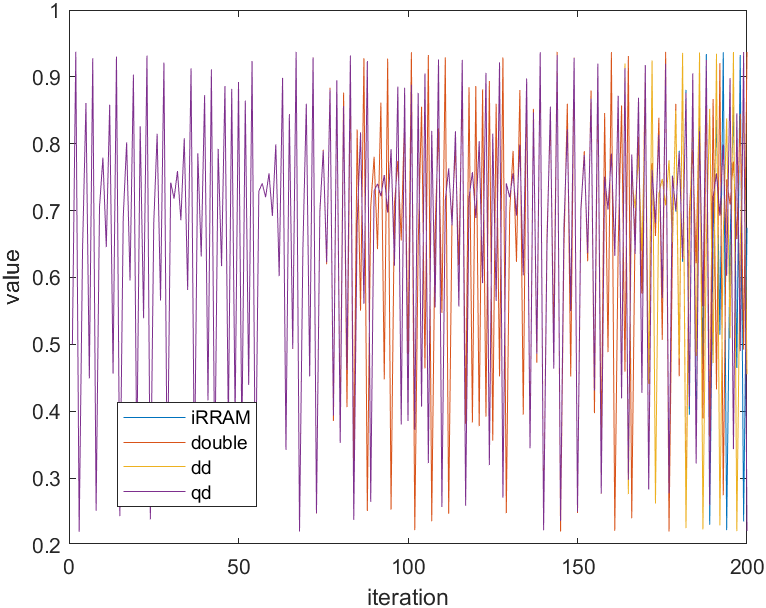
\includegraphics[scale=0.95]{img/1-1}\caption{raw values}
\end{figure}

You probably want to see clear disparity, or error.

\begin{figure}[H]
\centering{}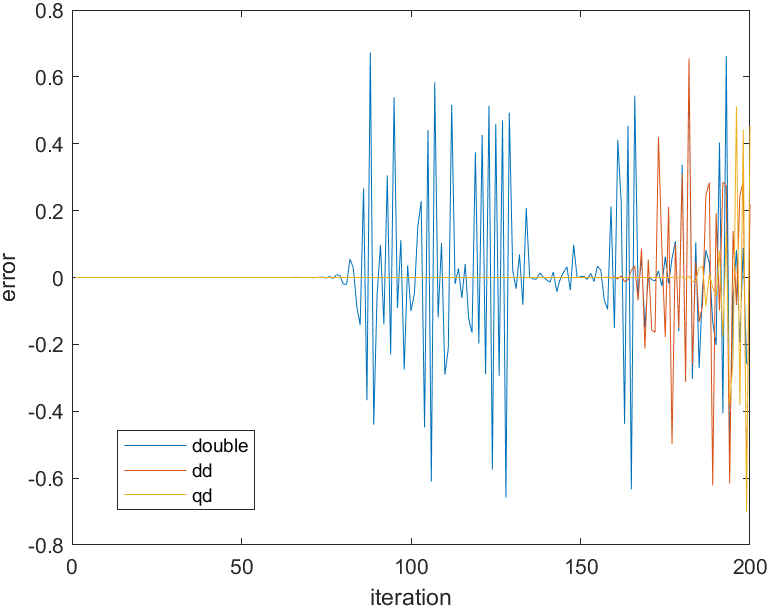
\includegraphics[scale=0.95]{img/1-2}\caption{errors}
\end{figure}

The first iteration \# at which err is greater than $\epsilon=0.000001$
are 55, 138, and 165 for Double, DD, and QD, respectively. Surprisingly,
from Double to DD, more than double iterations has been proceeded
with relatively low error. However, from DD to QD, only 27 more steps
were extended, even if both transitions make storage size double.

\section{Speed}

We analyzed for some basic opertions. Each operation is applied repeatedly
and we measure the elapsed time. This must not break correctness,
thereby, we first check if the value is correct, and then do the test.
Also, we repeated each experiment at least $2^{10}$times and took
the average because outliers came up out of blue. Lastly, when the
data seem to make a line, we made a linear regression on them.

\begin{algorithm}[H]
\begin{lstlisting}[language={C++},numbers=left,showstringspaces=false]
// iRRAM
for(int i=0;i<m;i++) {
  beginTime = high_resolution_clock::now();	// start timer
  r = rInit;
  for(long i=0;i<nPlus;i++) r = sqrt(r);	// apply the operation
  endTime = high_resolution_clock::now();	// stop timer
  rElapsed += duration_cast<nanoseconds>(endTime-beginTime).count(); // elapsed time
}
rElapsed /= m;		// take the average
\end{lstlisting}

\caption{Part of code for addition performance test}
\end{algorithm}

\newpage{}

\subsection{Addition}

Test setup: $x_{n+1}=x_{n}+c,\;x_{0}=1.0,c=3.14159,\;\left|e_{n}\right|<2^{-20}$

\begin{figure}[H]
\centering{}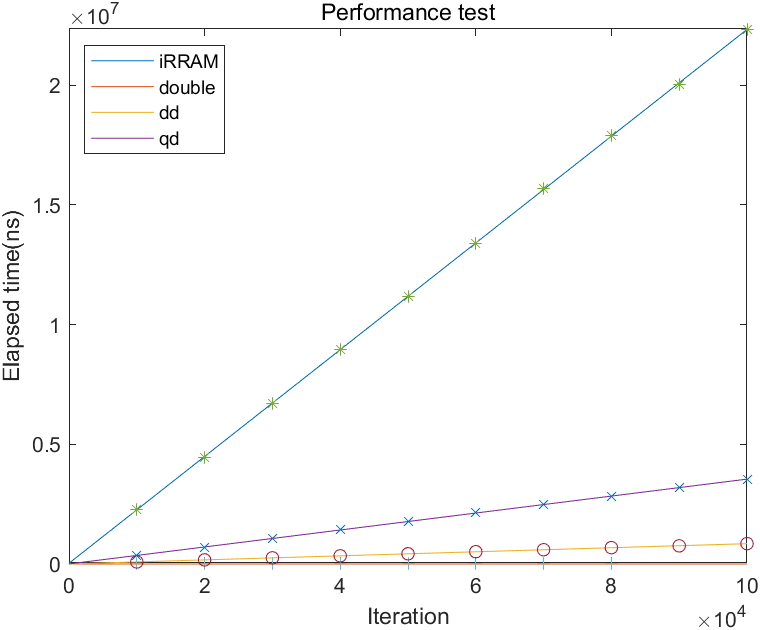
\includegraphics[scale=0.95]{img/2-1}\caption{Addition Test}
\end{figure}

\begin{table}[H]
\begin{tabular}{|c|c|c|c|c|}
\hline 
itr & iRRAM & double & DD & QD\tabularnewline
\hline 
\hline 
10000 & 2277466 & 40 & 85559 & 352622\tabularnewline
\hline 
20000 & 4464846 & 61 & 171552 & 706488\tabularnewline
\hline 
30000 & 6706339 & 59 & 255780 & 1070855\tabularnewline
\hline 
40000 & 8975040 & 40 & 341247 & 1426889\tabularnewline
\hline 
50000 & 11187951 & 51 & 426594 & 1774732\tabularnewline
\hline 
60000 & 13375699 & 47 & 513372 & 2134957\tabularnewline
\hline 
70000 & 15690342 & 39 & 595202 & 2500221\tabularnewline
\hline 
80000 & 17920073 & 39 & 682645 & 2807334\tabularnewline
\hline 
90000 & 20019130 & - & 758295 & 3203934\tabularnewline
\hline 
100000 & 22350155 & - & 849898 & 3541002\tabularnewline
\hline 
\end{tabular}%
\begin{tabular}{|c|c|c|c|c|}
\hline 
 & iRRAM & double & DD & QD\tabularnewline
\hline 
\hline 
slope & 223 & -0.0002 & 8.5 & 35.4\tabularnewline
\hline 
\end{tabular}
\centering{}\caption{Elapsed time(ns) and slope(ns/itr)}
\end{table}

Double is the fastest followed by DD, QD, and iRRAM. Double showed
a constant time complexity, but failed at iteration \# 89893 because
of lack of precision.

\newpage{}

\subsection{Multiplication}

Test setup: $x_{n+1}=x_{n}c,\;x_{0}=1.0,c=3.14159,\;\left|e_{n}\right|<2^{-20}$

\begin{figure}[H]
\centering{}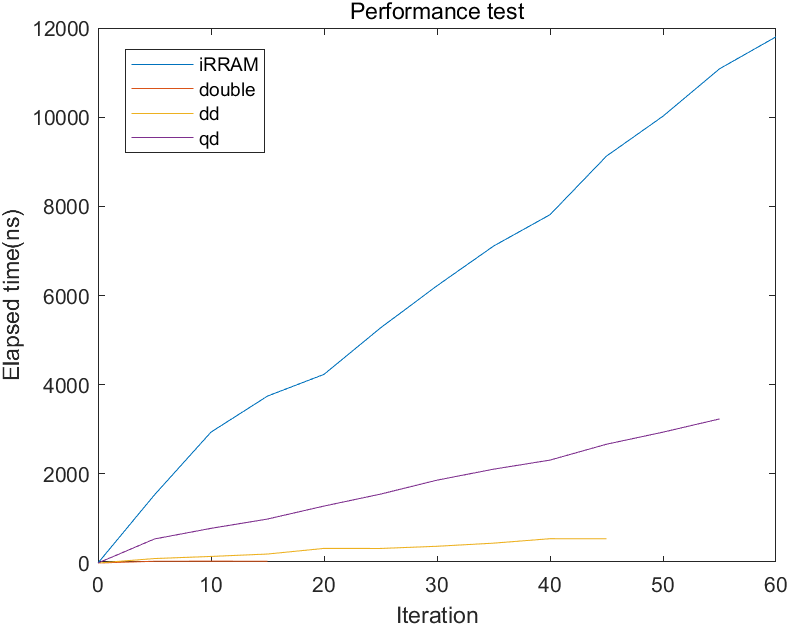
\includegraphics[scale=0.95]{img/2-2}\caption{Multiplication Test}
\end{figure}

\begin{table}[H]
\begin{tabular}{|c|c|c|c|c|}
\hline 
itr & iRRAM & double & DD & QD\tabularnewline
\hline 
\hline 
5 & 1207 & 43 & 90 & 253\tabularnewline
\hline 
10 & 2164 & 40 & 162 & 466\tabularnewline
\hline 
15 & 3314 & 40 & 201 & 728\tabularnewline
\hline 
20 & 4575 & - & 248 & 898\tabularnewline
\hline 
25 & 4954 & - & 316 & 1058\tabularnewline
\hline 
30 & 6190 & - & 441 & 1388\tabularnewline
\hline 
35 & 7033 & - & 467 & 1411\tabularnewline
\hline 
40 & 7952 & - & 500 & 1606\tabularnewline
\hline 
45 & 8960 & - & 571 & 1803\tabularnewline
\hline 
50 & 10191 & - & - & 2016\tabularnewline
\hline 
55 & 10952 & - & - & 2296\tabularnewline
\hline 
60 & 11834 & - & - & -\tabularnewline
\hline 
\end{tabular}%
\begin{tabular}{|c|c|c|c|c|}
\hline 
 & iRRAM & double & DD & QD\tabularnewline
\hline 
\hline 
slope & 192.93 & -0.3000 & 12.210 & 38.926\tabularnewline
\hline 
\end{tabular}
\centering{}\caption{Elapsed time(ns) and slope(ns/itr)}
\end{table}

With dramatically reduced iterations, the same performance order was
shown up.

\newpage{}

\subsection{Sqrt\label{subsec:Sqrt}}

Test setup: $x_{n+1}=\sqrt{x_{n}},\;x_{0}=3.14159,\;\left|e_{n}\right|<2^{-70}$

\begin{figure}[H]
\centering{}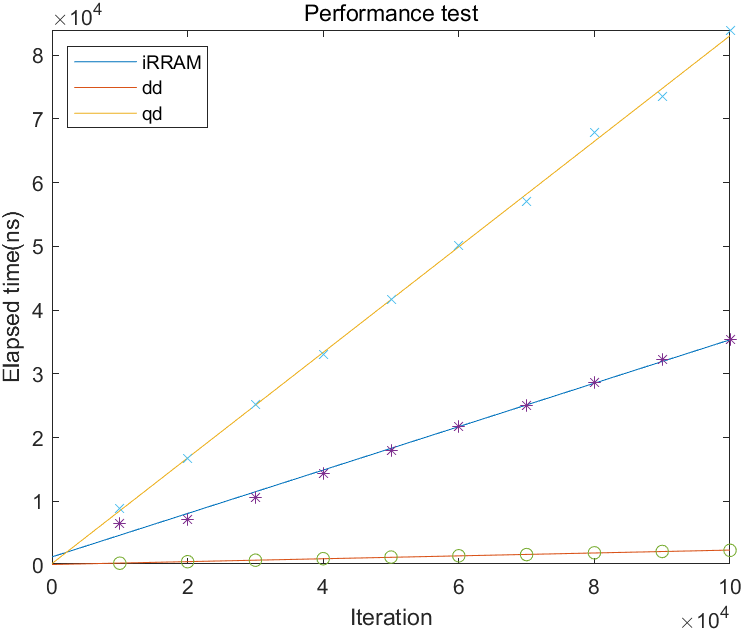
\includegraphics[scale=0.95]{img/2-3}\caption{Sqrt Test}
\end{figure}

\begin{table}[H]
\begin{tabular}{|c|c|c|c|c|}
\hline 
itr & iRRAM & double & DD & QD\tabularnewline
\hline 
\hline 
10 & 6576 & - & 280 & 8824\tabularnewline
\hline 
20 & 7204 & - & 518 & 16734\tabularnewline
\hline 
30 & 10624 & - & 752 & 25149\tabularnewline
\hline 
40 & 14309 & - & 986 & 33089\tabularnewline
\hline 
50 & 18002 & - & 1245 & 41635\tabularnewline
\hline 
60 & 21792 & - & 1447 & 50126\tabularnewline
\hline 
70 & 25075 & - & 1635 & 56960\tabularnewline
\hline 
80 & 28702 & - & 1912 & 67796\tabularnewline
\hline 
90 & 32293 & - & 2125 & 73445\tabularnewline
\hline 
100 & 35448 & - & 2300 & 83925\tabularnewline
\hline 
\end{tabular}%
\begin{tabular}{|c|c|c|c|c|}
\hline 
 & iRRAM & double & DD & QD\tabularnewline
\hline 
\hline 
slope & 340.6 & - & 22.653 & 828.02\tabularnewline
\hline 
\end{tabular}
\centering{}\caption{Elapsed time(ns) and slope(ns/itr)}
\end{table}

double couldn't produce any correct answer. iRRAM outperformed QD.
Maybe sqrt for QD is poorly implemented.

\newpage{}

\subsection{Sin}

Test setup: $x_{n+1}=\sin x_{n},\;x_{0}=3.14159,\;\left|e_{n}\right|<2^{-20}$

\begin{figure}[H]
\centering{}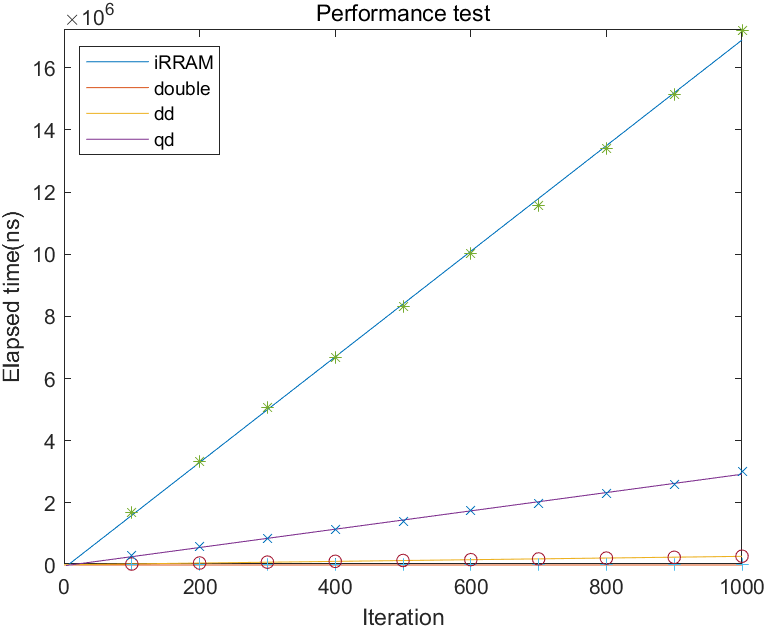
\includegraphics[scale=0.95]{img/2-4}\caption{$\sin$ Test}
\end{figure}

\begin{table}[H]
\begin{tabular}{|c|c|c|c|c|}
\hline 
itr & iRRAM & double & DD & QD\tabularnewline
\hline 
\hline 
100 & 1681688 & 53 & 31403 & 291835\tabularnewline
\hline 
200 & 3346861 & 53 & 63817 & 584602\tabularnewline
\hline 
300 & 5080634 & 56 & 92358 & 867127\tabularnewline
\hline 
400 & 6676655 & 40 & 118339 & 1138493\tabularnewline
\hline 
500 & 8311261 & 40 & 144700 & 1411165\tabularnewline
\hline 
600 & 10034068 & 40 & 171408 & 1748068\tabularnewline
\hline 
700 & 11581949 & 54 & 194743 & 1984476\tabularnewline
\hline 
800 & 13409914 & 53 & 222295 & 2316362\tabularnewline
\hline 
900 & 15135516 & 39 & 247799 & 2602703\tabularnewline
\hline 
1000 & 17218219 & 40 & 282751 & 3000588\tabularnewline
\hline 
\end{tabular}%
\begin{tabular}{|c|c|c|c|c|}
\hline 
 & iRRAM & double & DD & QD\tabularnewline
\hline 
\hline 
slope & 17000 & -0.0114 & 270 & 2947\tabularnewline
\hline 
\end{tabular}
\centering{}\caption{Elapsed time(ns) and slope(ns/itr)}
\end{table}

In the last part of iRRAM curve, there is a subtle performance improvement.
This is because of the error on measurement. The cpu must have done
something else during iteration \# 900 case, which had effect on the
elapsed time.

\newpage{}

\subsection{Euler Number (e=2.71...)}

In previous cases, each data structure produces true value until the
roundoff error takes place. On the other hand, this case produces
only approximation of $e$ at every iteration. So, let us change the
strategy. We set precision $p$ and aims $\left|x_{n}-e\right|\leq2^{p}$.
Because double, DD, and QD cannot have different limited precisions,
we proceed the experiments with different precisions for each data
structure, namely, $p_{m}\leq p<0$ where $p_{m}=-15$ for double,
$p_{m}=-97$ for DD, and $p_{m}=-196$ for QD.

Now that we are given a precision $p$, how do we approximate $e$?
We know

\begin{equation}
e=\sum_{k=0}^{n}\frac{1}{k!}+E_{n}\label{eq:e_taylor}
\end{equation}

where error $E_{n}$ is

\begin{equation}
E_{n}=\sum_{k=n+1}^{\infty}\frac{1}{k!}
\end{equation}

But

\begin{align*}
E_{n}= & \frac{1}{\left(n+1\right)!}+\frac{1}{\left(n+2\right)!}+\frac{1}{\left(n+3\right)!}+\cdots\\
= & \frac{1}{\left(n+1\right)!}\left[1+\frac{1}{\left(n+2\right)}+\frac{1}{\left(n+2\right)\left(n+3\right)}+\cdots\right]\\
\leq & \frac{1}{\left(n+1\right)!}\left[1+\frac{1}{1}+\frac{1}{1\times2}+\frac{1}{1\times2\times3}\cdots\right]\\
= & \frac{e}{\left(n+1\right)!}
\end{align*}

Meanwhile, $\frac{e}{n+1}\leq2$ for $n\geq1$. By multiplying $1/n!$
on both hands,

\begin{equation}
\left|E_{n}\right|=\frac{e}{\left(n+1\right)!}\leq\frac{2}{n!}
\end{equation}

Therefore, we keep adding up $1/k!$ from $\text{\eqref{eq:e_taylor}}$
until $2/n!\leq2^{p}$ is satisfied.

\subsubsection{iRRAM vs double}

\begin{figure}[H]
\centering{}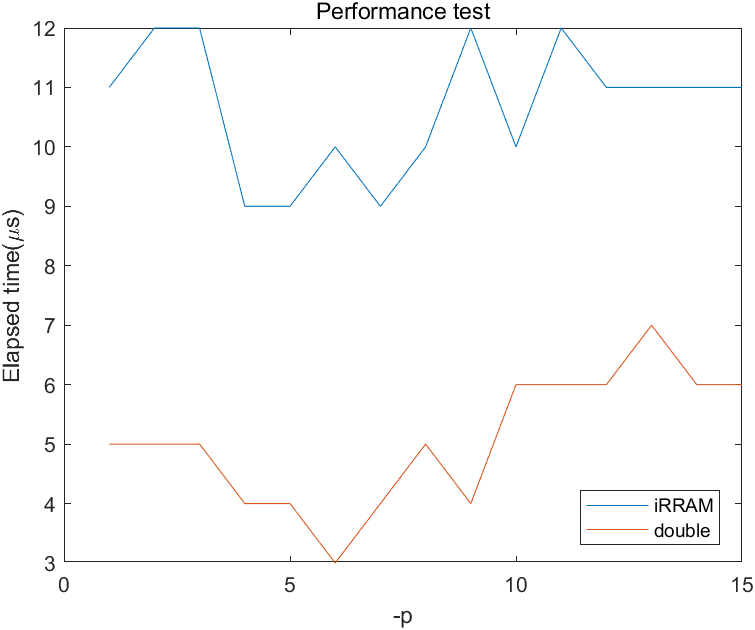
\includegraphics[scale=0.95]{img/2-5-1}\caption{Runtime: iRRAM vs double}
\end{figure}

\begin{table}[H]
\begin{tabular}{|c|c|c|}
\hline 
-p & iRRAM & double\tabularnewline
\hline 
\hline 
1 & 11 & 5\tabularnewline
\hline 
2 & 12 & 5\tabularnewline
\hline 
3 & 12 & 5\tabularnewline
\hline 
4 & 9 & 4\tabularnewline
\hline 
5 & 9 & 4\tabularnewline
\hline 
6 & 10 & 3\tabularnewline
\hline 
7 & 9 & 4\tabularnewline
\hline 
8 & 10 & 5\tabularnewline
\hline 
9 & 12 & 4\tabularnewline
\hline 
10 & 10 & 6\tabularnewline
\hline 
11 & 12 & 6\tabularnewline
\hline 
12 & 11 & 6\tabularnewline
\hline 
13 & 11 & 7\tabularnewline
\hline 
14 & 11 & 6\tabularnewline
\hline 
15 & 11 & 6\tabularnewline
\hline 
\end{tabular}
\centering{}\caption{Runtime: iRRAM vs double}
\end{table}

Note that x-axis indicates $-p$ instead of $p$. Double beats iRRAM.

\subsubsection{iRRAM vs double double}

\begin{figure}[H]
\centering{}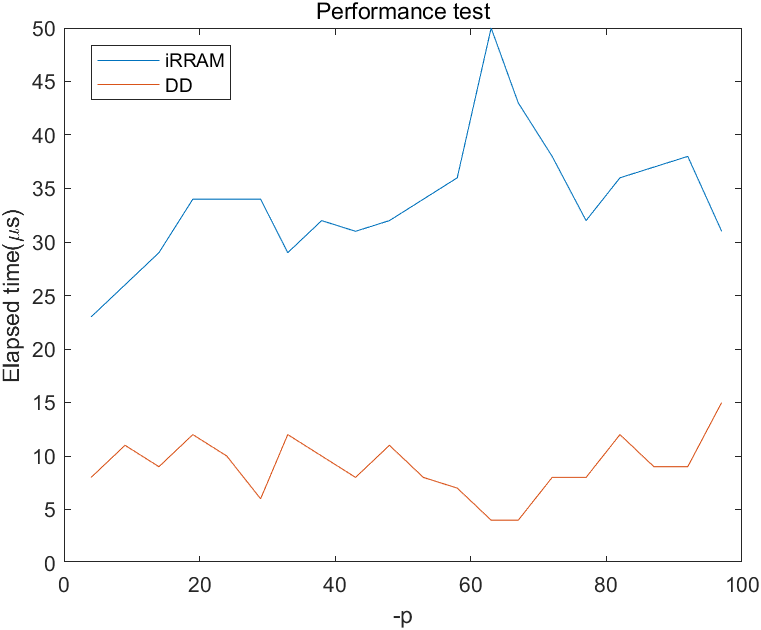
\includegraphics[scale=0.95]{img/2-5-2}\caption{Runtime: iRRAM vs DD}
\end{figure}

\begin{table}[H]
\begin{tabular}{|c|c|c|}
\hline 
-p & iRRAM & DD\tabularnewline
\hline 
\hline 
4 & 23 & 8\tabularnewline
\hline 
9 & 26 & 11\tabularnewline
\hline 
14 & 29 & 9\tabularnewline
\hline 
19 & 34 & 12\tabularnewline
\hline 
24 & 34 & 10\tabularnewline
\hline 
29 & 34 & 6\tabularnewline
\hline 
33 & 29 & 12\tabularnewline
\hline 
38 & 32 & 10\tabularnewline
\hline 
43 & 31 & 8\tabularnewline
\hline 
48 & 32 & 11\tabularnewline
\hline 
53 & 34 & 8\tabularnewline
\hline 
58 & 36 & 7\tabularnewline
\hline 
63 & 50 & 4\tabularnewline
\hline 
67 & 43 & 4\tabularnewline
\hline 
72 & 38 & 8\tabularnewline
\hline 
77 & 32 & 8\tabularnewline
\hline 
82 & 36 & 12\tabularnewline
\hline 
87 & 37 & 9\tabularnewline
\hline 
92 & 38 & 9\tabularnewline
\hline 
97 & 31 & 15\tabularnewline
\hline 
\end{tabular}
\centering{}\caption{Runtime: iRRAM vs DD}
\end{table}

Once again, DD beats iRRAM.

\subsubsection{iRRAM vs quad double\label{subsec:iRRAM-vs-quad}}

\begin{figure}[H]
\centering{}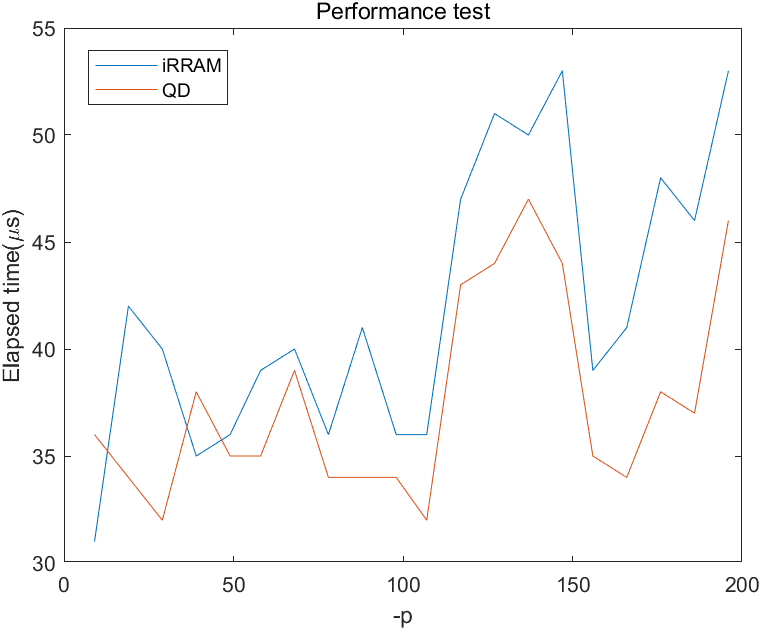
\includegraphics[scale=0.95]{img/2-5-3}\caption{Runtime: iRRAM vs QD}
\end{figure}

\begin{table}[H]
\begin{tabular}{|c|c|c|}
\hline 
-p & iRRAM & QD\tabularnewline
\hline 
\hline 
9 & 31 & 36\tabularnewline
\hline 
19 & 42 & 34\tabularnewline
\hline 
29 & 40 & 32\tabularnewline
\hline 
39 & 35 & 38\tabularnewline
\hline 
49 & 36 & 35\tabularnewline
\hline 
58 & 39 & 35\tabularnewline
\hline 
68 & 40 & 39\tabularnewline
\hline 
78 & 36 & 34\tabularnewline
\hline 
88 & 41 & 34\tabularnewline
\hline 
98 & 36 & 34\tabularnewline
\hline 
107 & 36 & 32\tabularnewline
\hline 
117 & 47 & 43\tabularnewline
\hline 
127 & 51 & 44\tabularnewline
\hline 
137 & 50 & 47\tabularnewline
\hline 
147 & 53 & 44\tabularnewline
\hline 
156 & 39 & 35\tabularnewline
\hline 
166 & 41 & 34\tabularnewline
\hline 
176 & 48 & 38\tabularnewline
\hline 
186 & 46 & 37\tabularnewline
\hline 
196 & 53 & 46\tabularnewline
\hline 
\end{tabular}
\centering{}\caption{Runtime: iRRAM vs QD}
\end{table}

This looks pretty different. First, the difference isn't as big as
those of the previous cases. Second, there are some sections on which
iRRAM runs faster than QD especially on $-p\in\left(0,50\right)$.
Whenever we do this experiment, the graph changes. However, these
two remarks never change. It is another clue to doubt the implementaion
of QD along with Sec $\text{\ref{subsec:Sqrt}}$.

\section{Conclusion}

We couldn't see the break-even point. Double and DD outperformed iRRAM
for all experiments. In addition, QD showed slower performance than
iRRAM does at Sec $\text{\ref{subsec:Sqrt}}$, or similar performance
at Sec $\text{\ref{subsec:iRRAM-vs-quad}}$. Therefore it is efficient
to use double, DD, and QD if the desired precision is small enough
for those data structure except sqrt.

\bibliographystyle{plain}
\bibliography{my}

\end{document}
